\section{Provenance}
In the Oxford dictionary, \emph{provenance} is defined as ``the place of origin or earliest known history of something''. Provenance plays an important role in many aspects of our daily lives. For example, in everyday shopping, before purchasing a bottle of fruit juice, a customer would like to know about its origin, ingredients, methods of collecting, storing and processing fruits, etc. In art, the provenance information of a painting such as authorship, material, painting time and the story behind the painting greatly decides its value. In computer systems, the provenance of a piece of data is defined as ``the process that led to that piece of data''~\cite{Moreau2011}. It contains information about the input data, the output data, and the configuration of the program used to process the data.

Provenance can be broadly categorized into two groups. The first group, \emph{data provenance}, relies on the previous definition of provenance in computer systems, focusing on the derivation history of data including its source information and the process that produced it. This type of provenance is often emphasized in data-intensive fields such as scientific workflows and databases. The second group, \emph{analytic provenance}, is usually mentioned in the context of visualization and sensemaking. It focuses on the interactive data exploration and the reasoning process driven by sensemaking including the provenance of visualizations used, interactions performed, analytical insights found and the conclusion and rationale behind them. Next, we discuss data provenance in different fields that are active in provenance research, including scientific workflows, databases and semantic webs. Then, we will follow with the review of analytic provenance.

\subsection{Data Provenance}
\label{sub:lr-data-provenance}
Scientific experiments may consist of thousands of steps, with each step involving distributed data sources and computational data models~\cite{Gil2007}. Workflows have been used to facilitate the assembly, automation and management of such experiments. Notable scientific workflow systems with provenance enabled include Tarvena~\cite{Zhao2008}, Kepler~\cite{Bowers2006} and VisTrails~\cite{Bavoil2005}. Provenance plays an important role in scientific workflows, aiming to support data interpretation, reproduction of experiment results, troubleshooting and optimization~\cite{Miles2007}. Zhao, Wilde and Foster~\cite{Zhao2006} discuss two types of provenance in workflows: \emph{prospective provenance} -- focusing on the workflow design, and \emph{retrospective provenance} -- focusing on the workflow execution. The provenance of long and complex workflows is huge, thus posing challenges in storing, querying, and making sense of such data~\cite{Davidson2007}.

Curated databases are populated and updated with a great deal of human effort, typically published on the web~\cite{Buneman2008}. A well-known example is Wikipedia -- a free Internet encyclopedia that allows its users to edit almost all articles. Each record in these curated databases, such as a Wikipedia article, may be edited by many users and referred to other internal and external sources. This produces problems in attribution and provenance: who edited what and when. Research in database provenance can be characterized into a why-where-how framework~\cite{Cheney2007}. \emph{Why}-provenance focuses on the lineage of the output: for each tuple $t$ in the output, the lineage of $t$ is a set of tuples in the input data that produces $t$~\cite{Cui2000}. \emph{How}-provenance concerns how the output tuple $t$ is derived from the query~\cite{Green2007}. Finally, \emph{where}-provenance describes specific locations, or cells in relational databases, of the input data that contributes to the query output~\cite{Buneman2001}. To compute these types of provenance, two general approaches have been introduced~\cite{Buneman2008}. An \emph{eager} approach adjusts the query to pass the extra provenance information to the output. Whereas, a \emph{lazy} approach computes provenance on demand.

Data provenance research in scientific workflows and databases so far has mainly focused on closed systems, which have full access to the data and its provenance. Modern applications with service-oriented and cloud-computing architectures bring challenges in tracking and exchanging provenance information across systems. The \emph{Open Provenance Model} is designed to address these challenges~\cite{Moreau2011}. It also supports a digital representation of provenance for any objects, whether produced by computer systems or not. Three types of objects are defined in the model for building this representation. An \emph{artifact} is a state that can be a digital or physical object. A \emph{process} is a series of actions performed on or caused by artifacts, and resulting in new artifacts. An \emph{agent} acts as a catalyst of the process, managing its execution. Different types of causal relationships can be added between these nodes, forming a \emph{provenance graph} as shown in \autoref{fig:lr-provenance-graph}.

\begin{figure}
	\centering
	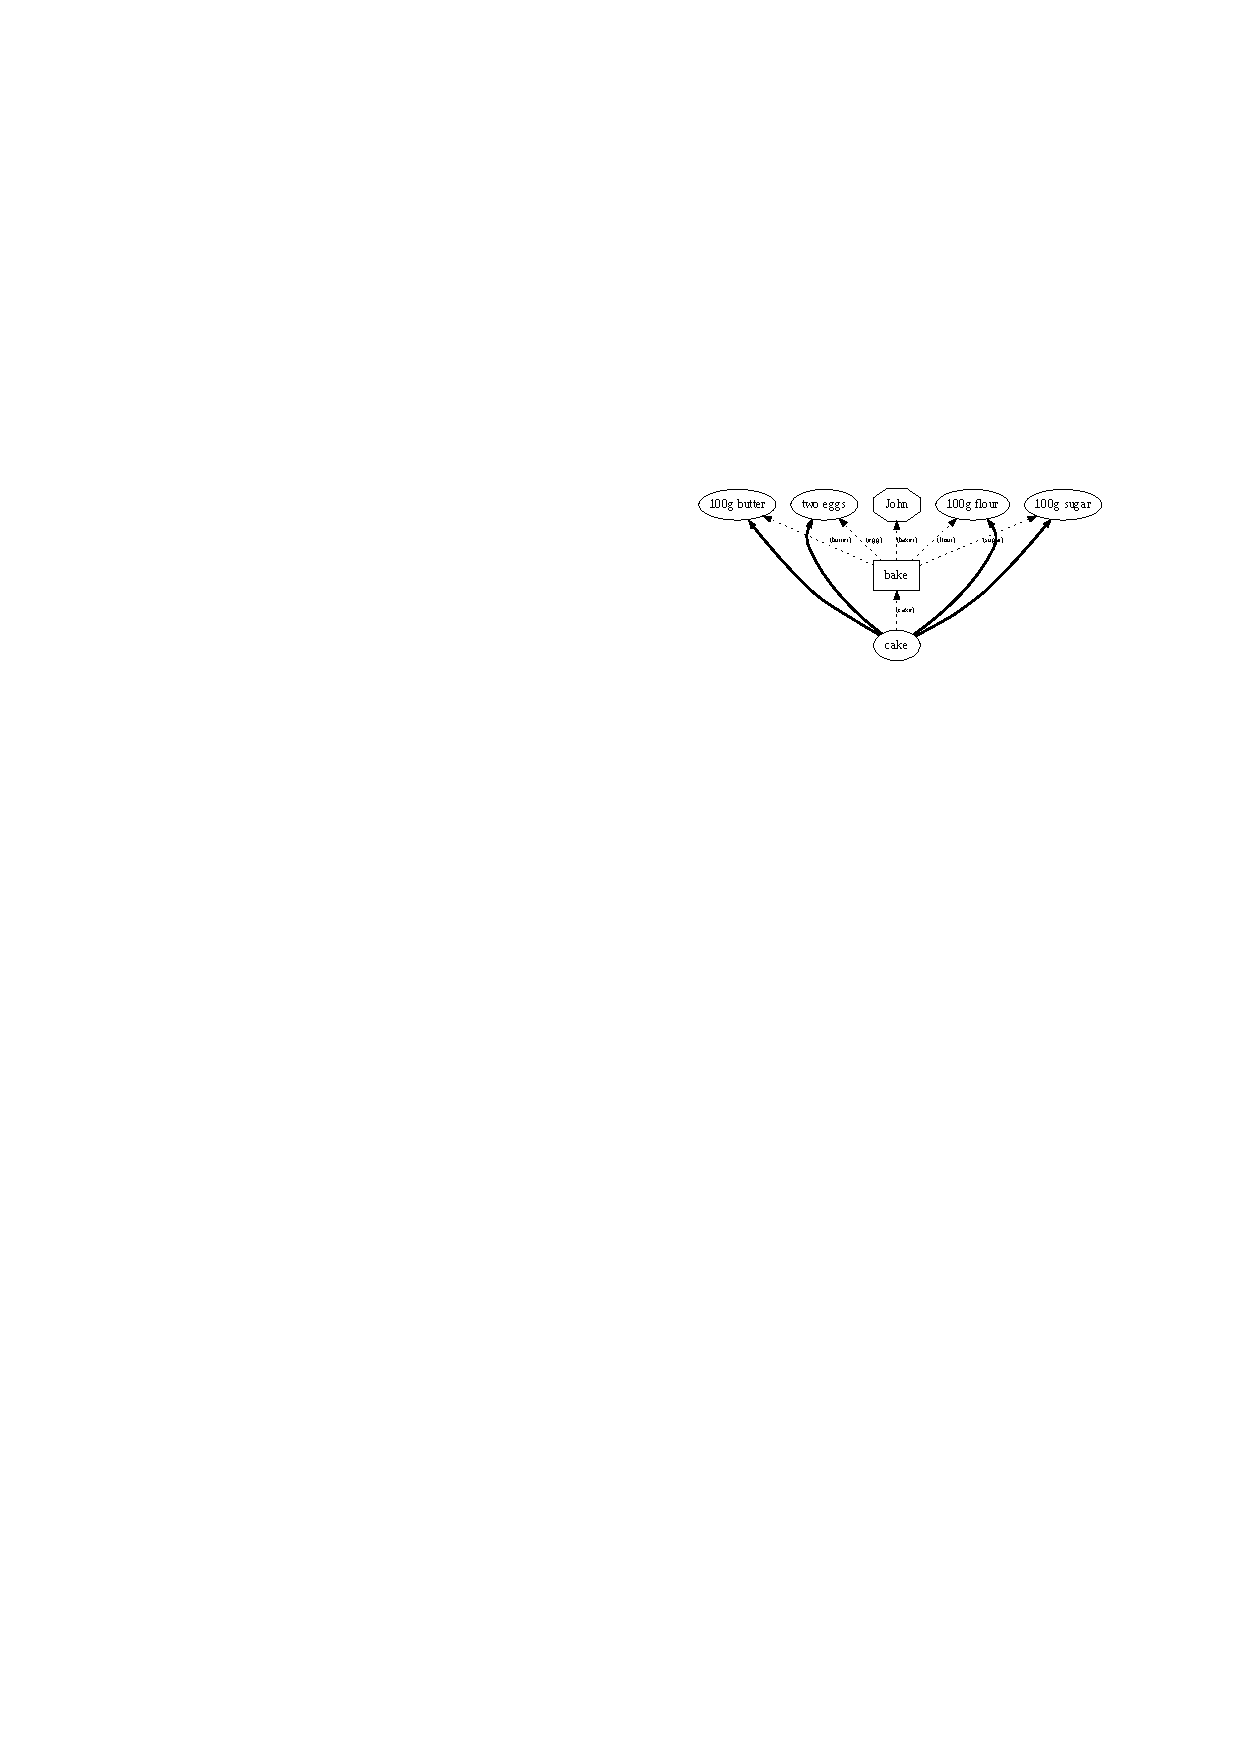
\includegraphics[width=.8\linewidth]{provenance-graph}
	\caption[An example of provenance graph]{A provenance graph for ``cake baking'' using the Open Provenance Model. The cake (artifact) was baked (the process) by John (the agent) using ingredients (artifacts) including butter, eggs, flour and sugar. \is{Moreau2011}}
	\label{fig:lr-provenance-graph}
\end{figure}

The Open Provenance Model has been implemented in many different scientific workflow systems such as Tarvena~\cite{Zhao2008}, Kepler~\cite{Bowers2006} and VisTrails~\cite{Bavoil2005}. The model is general and can be extended in both the structure and vocabulary to represent domain-specific problems. \emph{D-profile}~\cite{Groth2011} describes an extension of the model for representing provenance in distributed systems. ProveML~\cite{Walker2013} is an extension for recording the provenance of data, analytical process and interpretation in human terrain visual analytics.

The \emph{PROV} set of specifications, produced by the World Wide Web Consortium, is designed to promote the publication of provenance information on the Web and support the interchange of provenance across diverse provenance management systems~\cite{Missier2013}. The PROV-DM is the conceptual data model that forms a basis of PROV and is based on the aforementioned open provenance model. Besides the core data model, PROV also includes other extensions such as PROV-CONSTRAINTS, a set of constraints applied to the data model to impose rules for consistency and validity of provenance.

\subsection{Analytic Provenance}
\label{sec:lr-analytic-provenance}
Analytic provenance focuses on understanding the sensemaking process of a user through the study of his or her interaction with a visualization~\cite{North2011}. It captures both the interactive data exploration process and the accompanied human reasoning process during sensemaking~\cite{Xu2015}. This section discusses models for representing analytic provenance data, methods to capture the data and techniques to visualize the captured data for supporting sensemaking.

\subsubsection{Model}
\label{sec:lr-analytic-provenance-model}
Analytic provenance information can be categorized using a four-layer hierarchical model based on its semantic richness proposed by Gotz and Zhou~\cite{Gotz2009}. \autoref{fig:lr-Gotz-Zhou-model} illustrates this model with the level of semantics increasing from bottom to top. The bottom-level \emph{events} consist of low-level user interaction such as mouse clicks and keystrokes, which contain little semantic meaning. The next level up includes \emph{actions}, which are analytic steps such as querying the database or changing the zooming level of a data visualization. The parameters such as data description and visualization settings are also part of the provenance. Further up are the \emph{sub-tasks}, which are the analyses required to achieve the sensemaking goal. Considering stock market analysis as the top-level \emph{task}, examples of sub-tasks could be identifying top performing companies and long term trends.

\begin{figure}
	\centering
	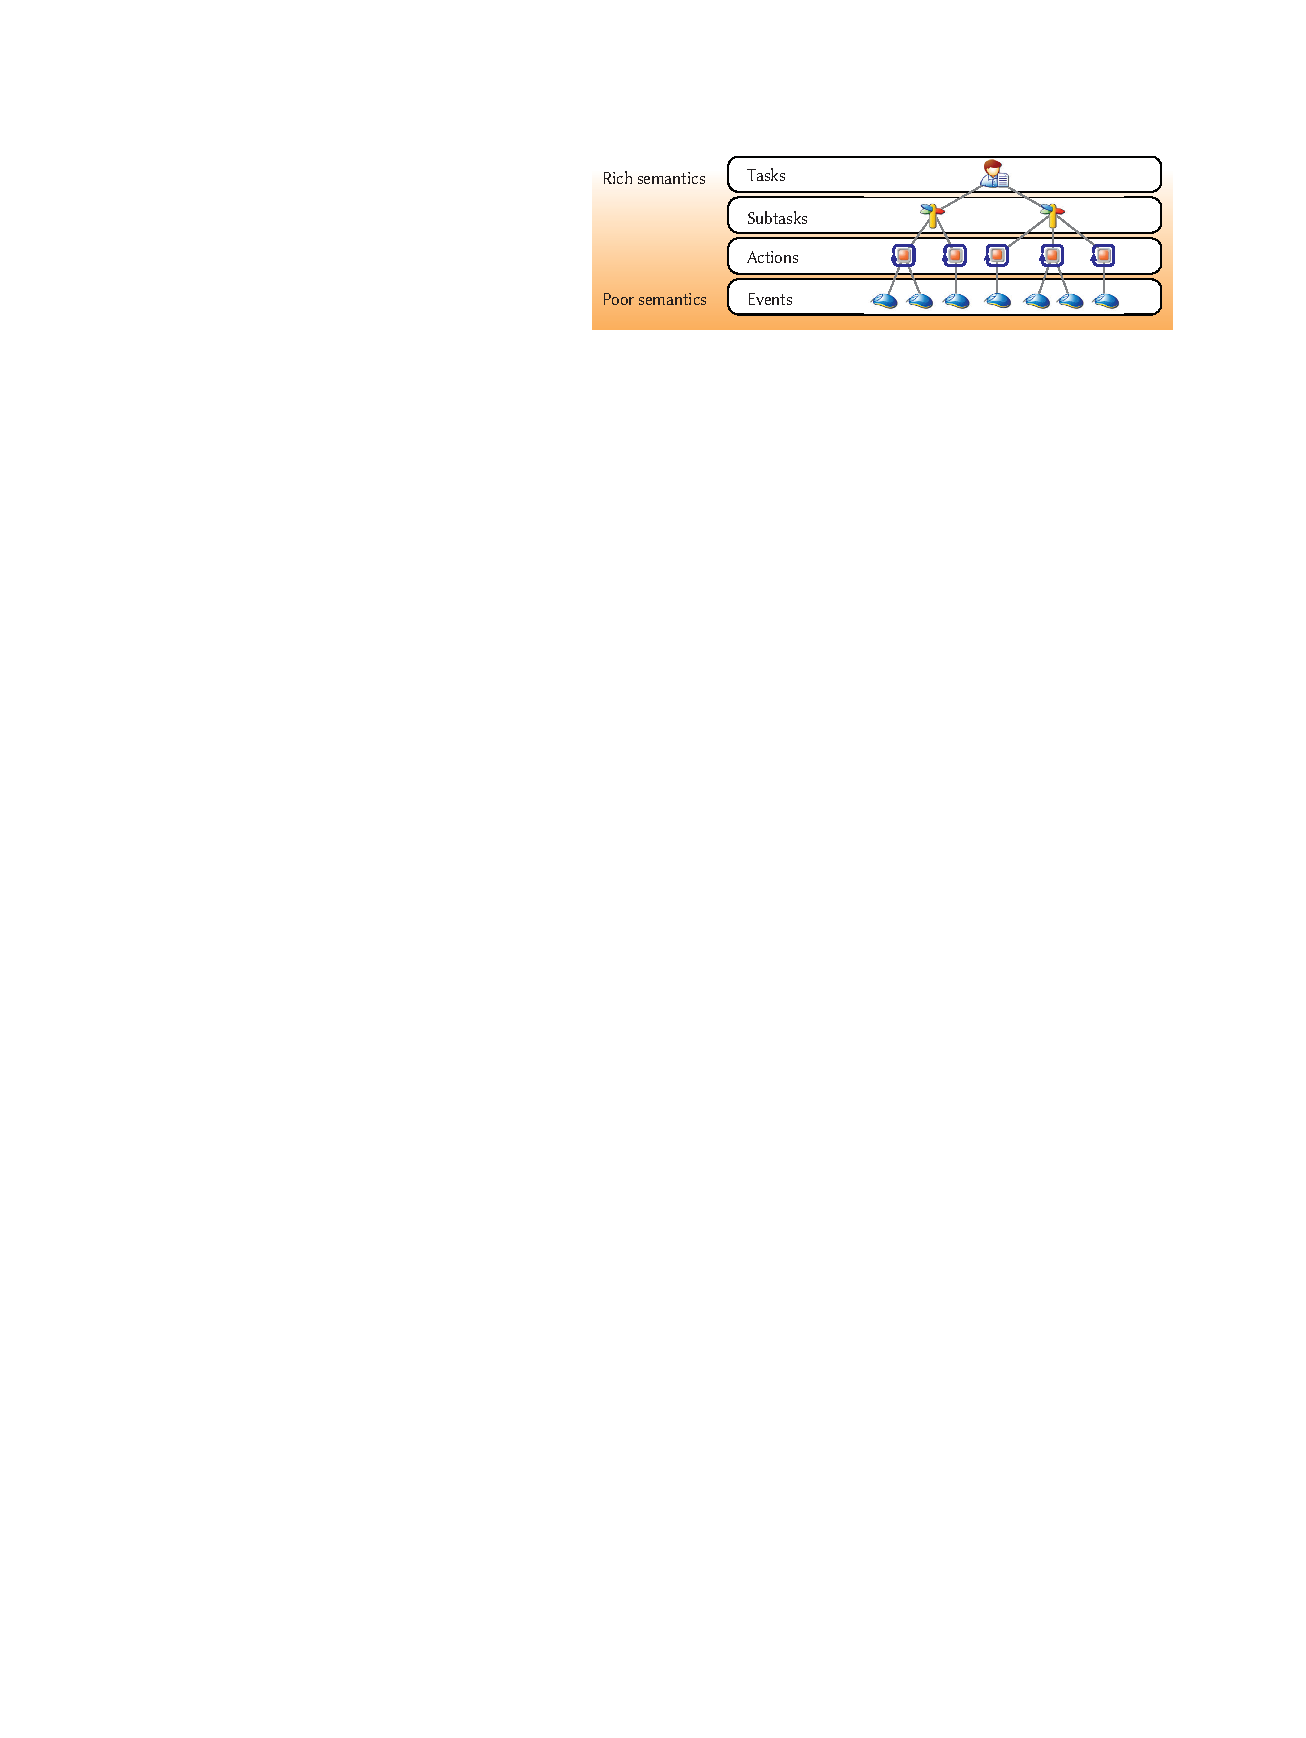
\includegraphics[width=.8\columnwidth]{Gotz-Zhou-model}
	\caption[The four-level semantic provenance model]{The hierarchical analytic provenance model with semantic richness increasing from bottom to top. The bottom layer includes \emph{events} such as key presses and mouse clicks, which have little semantics. The next level up contains \emph{actions} such as the database query and visualization zooming. Further up level consists of \emph{sub-tasks}, which usually are the analyses performed during the sensemaking. The top level \emph{tasks} are the overall sensemaking undertaking. \is{Gotz2009}}
	\label{fig:lr-Gotz-Zhou-model}
\end{figure}

Analytic provenance is closely linked both within and across layers. Within a layer, analytic provenance is linked temporally (i.e., one event happens after another) and logically (e.g., one action depends on the two previous actions). A sequence of elements in each layer is performed to serve for a higher semantic element in the above layer. For example, a database query action consists of several mouse click and key stroke events, and it can be part of a higher level sub-task such as ``comparing stock performance''.

This four-layer model is general, allowing the designers to determine the specific elements they want to capture within each layer for their systems. For example, many existing taxonomies of visualization interaction and tasks~\cite{Amar2005, Gotz2009} can be used to guide the selection in \emph{action} and \emph{sub-task} layers. Low-level analytic activities such as ``retrieve value'', ``sort'' and ``filter'' can represent the \emph{action} layer. A taxonomy of interaction techniques based on their intent such as ``show me more related items'' may stay in-between the \emph{action} layer and \emph{sub-task} layer~\cite{Yi2007}. A multi-level typology of abstract visualization tasks by Brehmer and Munzner~\cite{Brehmer2013} distinguishes why and how a task is performed, as well as what the task input and output are. The \emph{how} part of this typology can be a good candidate for representing the \emph{action} layer, and the \emph{why} part can be suitable for the \emph{sub-task} layer.

A recent taxonomy by Ragan~et~al.~\cite{Ragan2016} characterizes provenance in visualization and analysis systems based on the type of provenance and the purpose of collecting it. Five ``flat'' provenance types include data, visualization, interaction, insight and rationale. The type of \emph{data} provenance is similar to the previous discussion in \autoref{sub:lr-data-provenance}. \emph{Visualization} provenance concerns with the history of graphical views and visualization states, and \emph{interaction} provenance focuses on the history of user actions within a system. The combination of these two types of provenance is equivalent to the \emph{action} layer in Gotz and Zhou's model. \emph{Insight} provenance describes the findings and \emph{rationale} provenance explains the reasoning process that led to these findings. These two types of provenance can be referred to the \emph{sub-task} layer.

The following sections categorize analytic provenance research into four layers of the Gotz and Zhou's model, focusing on the capture and visualization techniques for each layer.

\subsubsection{Events}

\paragraph{Capture}
There is limited literature on capturing events because it is relatively easy and provides little semantics. A notable example is Glass Box~\cite{Cowley2006}, which can record a wide range of low-level events such as mouse clicks, key strokes and window events. Its objective is to capture and archive intelligence analysis activities for later retrieval. Simply capturing these events alone is insufficient to understand their purpose and rationale. For example, even though we know that a \textit{mouse click} happened; however, what the purpose of that click was (e.g., to sort the data), and why the user performed that click (e.g., to find an interesting pattern from the data) are unknown. In data exploration with a visualization, an analyst often performs many operations and takes different approaches in order to find interesting patterns. In that case, a series of poor-semantic events makes it more difficult for the analyst to recall what has been done. Therefore, more meaningful activities are required to be captured together.

\paragraph{Visualization}
Because low-level events contain little semantics, they may not be able to immediately provide meaningful insight and near real-time support to the users during their sensemaking processes. However, in a post hoc analysis, they can be used to gain a deep understanding about the processes that took place. For example, a visualization of users' mouse clicks can reveal patterns of application usage~\cite{Matejka2013} and highlight important usability issues, such as pages where users spent a lot of time and pages where they got lost during the task~\cite{Waterson2002}. User interaction with visual analytics systems can be visually examined to recover their reasoning processes employed in their analysis tasks such as specific findings and strategies they used to discover them~\cite{Dou2009, Guo2016}. Interaction logs have also been used to predict user performance of basic visualization tasks like visual search~\cite{Brown2014}.

\subsubsection{Actions}

\paragraph{Capture}
During the data exploration with a visualization, all user interaction can be systematically recorded. The visual exploration process can be modeled using a \textit{graph} metaphor. Nodes in the graph represent \textit{states} of the visualization and edges represent \textit{actions} that transform one state into another state. A state includes all the information required to reconstruct the captured visualization. For example, a state of a \textit{scatter plot} may include the dataset, data attributes mapped to visual channels such as spatial positions, color and size. An action could be changing the size mapping. Commonly, undo and redo features are provided to allow revisiting to previous states. If a new action is performed from a past state, a new branch will be created to store that new line of actions.

Two common strategies can be applied to automatically capture the exploration process. The first strategy captures the initial state and all the actions so that they can be executed to reproduce all states~\cite{Kadivar2009}. This allows reapplication of the analysis process with a different dataset, but could be time-inefficient if the number of actions is high. The second strategy simply captures the visualization state after every action~\cite{Bavoil2005}. This is easier to implement, but may be memory-expensive if a state contains too much information.

In the context of everyday, online sensemaking, users interact with a standard web browser instead of a visualization system. These browsers often capture data about visited web pages including visit time, web titles, URLs and favorite icons. Linking relationship between pages such as opening from a web link and using the browser's back button can also be captured~\cite{Ayers1995,Hightower1998,Milic-Frayling2003}. This results in a hierarchical history rather than a linear list of visited web pages in browser's history feature. Manual capture through bookmarking is also a standard feature of web browsers, allowing users to save web pages for revisitation purpose. Besides bookmarking a whole web page through its URL, a page element such as \textit{table} and \textit{form} HTML tags~\cite{Hong2008}, and a specific fragment of text~\cite{Dontcheva2006} can also be saved. These more fine-grained captures allow users to record what they want with a higher accuracy.

\paragraph{Visualization}
We discuss different visual representations of actions and states, and different layouts to position them.

\subparagraph{Visual Representation}
The simplest representation is \textbf{text}, commonly used to describe actions and states, such as names of actions, titles of visited web pages and content of user notes. Text can provide accurate information, but long text makes it difficult for users to understand and recognize. A graphical browser history by Ayers and Stasko~\cite{Ayers1995} shortens web page titles to accommodate more pages in the view. Within a given width, its truncating method preserves complete words at both ends of the title and trims characters in the middle if necessary. Kaasten, Greenberg and Edwards~\cite{Kaasten2001} compare the recognizability of titles between various string sizes for all three truncation methods (text is truncated at the beginning, middle or end of the title). The results show that for a medium (60\%) recognition, 15 -- 20 letters (depending on
the truncation method) are required for recognizing web sites, and 28 -- 39 letters are required for recognizing exact pages. For longer text such as user notes, machine learning techniques for text summarization could be beneficial~\cite{Nenkova2012}.

\textbf{Icon} is another popular choice of visual representation for actions and states, enabling users to easily distinguish them. They can be used alone to represent the analysis process when the visual result of each action is out of interest (\autoref{fig:lr-action-1}). Alternatively, these icons can be used together with visualization states, connecting the one before and the one after an action (\autoref{fig:lr-action-2}).

\begin{figure}
\centering
\subcaptionbox{A sequence of icons representing the analysis process. \is{Gotz2009}\label{fig:lr-action-1}}[\columnwidth]{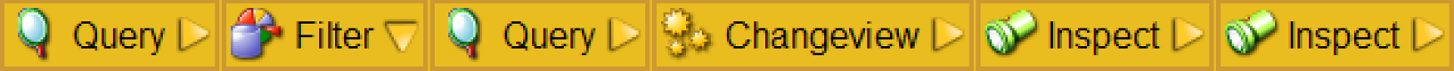
\includegraphics[width=.8\columnwidth]{action-1}}

\vspace{.5\baselineskip}

\subcaptionbox{Iconic actions connecting two visualization states. \is{Ma1999}\label{fig:lr-action-2}}[\columnwidth]{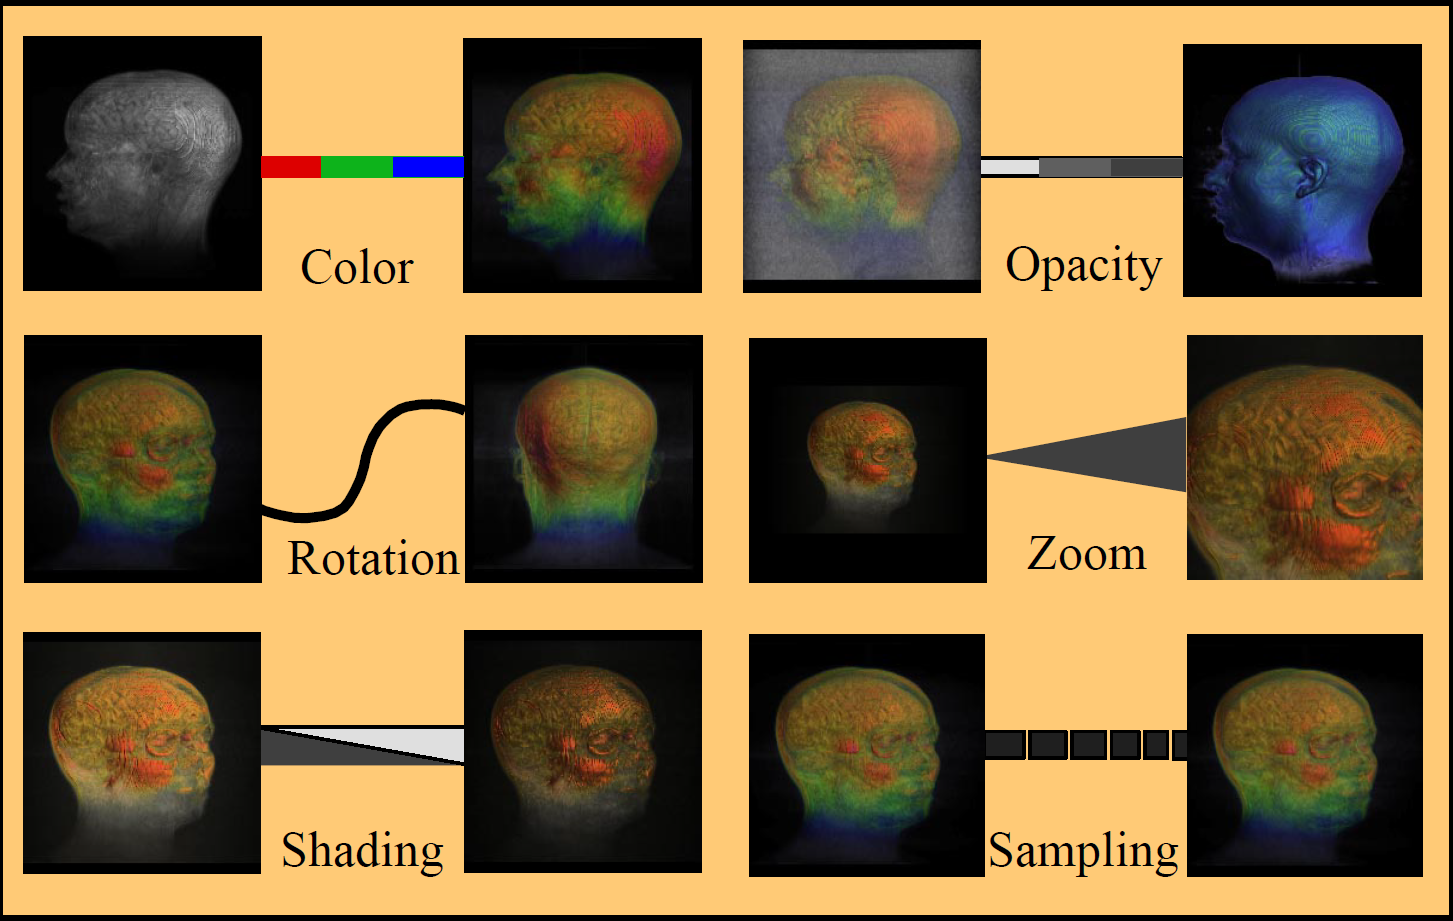
\includegraphics[width=.8\columnwidth]{action-2}}
\caption{Icons as visual representation of actions.}
\end{figure}

\textbf{Thumbnails} are commonly used to represent visualization states, aiding users' recognition of previous ones. One study suggests that a thumbnail size of 96 pixels square could provide 60\% accurate recognition of a visited web site~\cite{Kaasten2001}. For the same accuracy but in recognizing an exact web page, the thumbnail size rises to 144 pixels square. Additional information can be added to a web thumbnail to improve its recognition such as how often the represented page is revisited and whether that page is bookmarked or not~\cite{Cockburn1999}. For visualization thumbnails, visual encodings and parameters that were used to produce the visualization can also be embedded (\autoref{fig:lr-thumbnail-encoding}), providing more provenance information to the users.

\begin{figure}
	\centering
	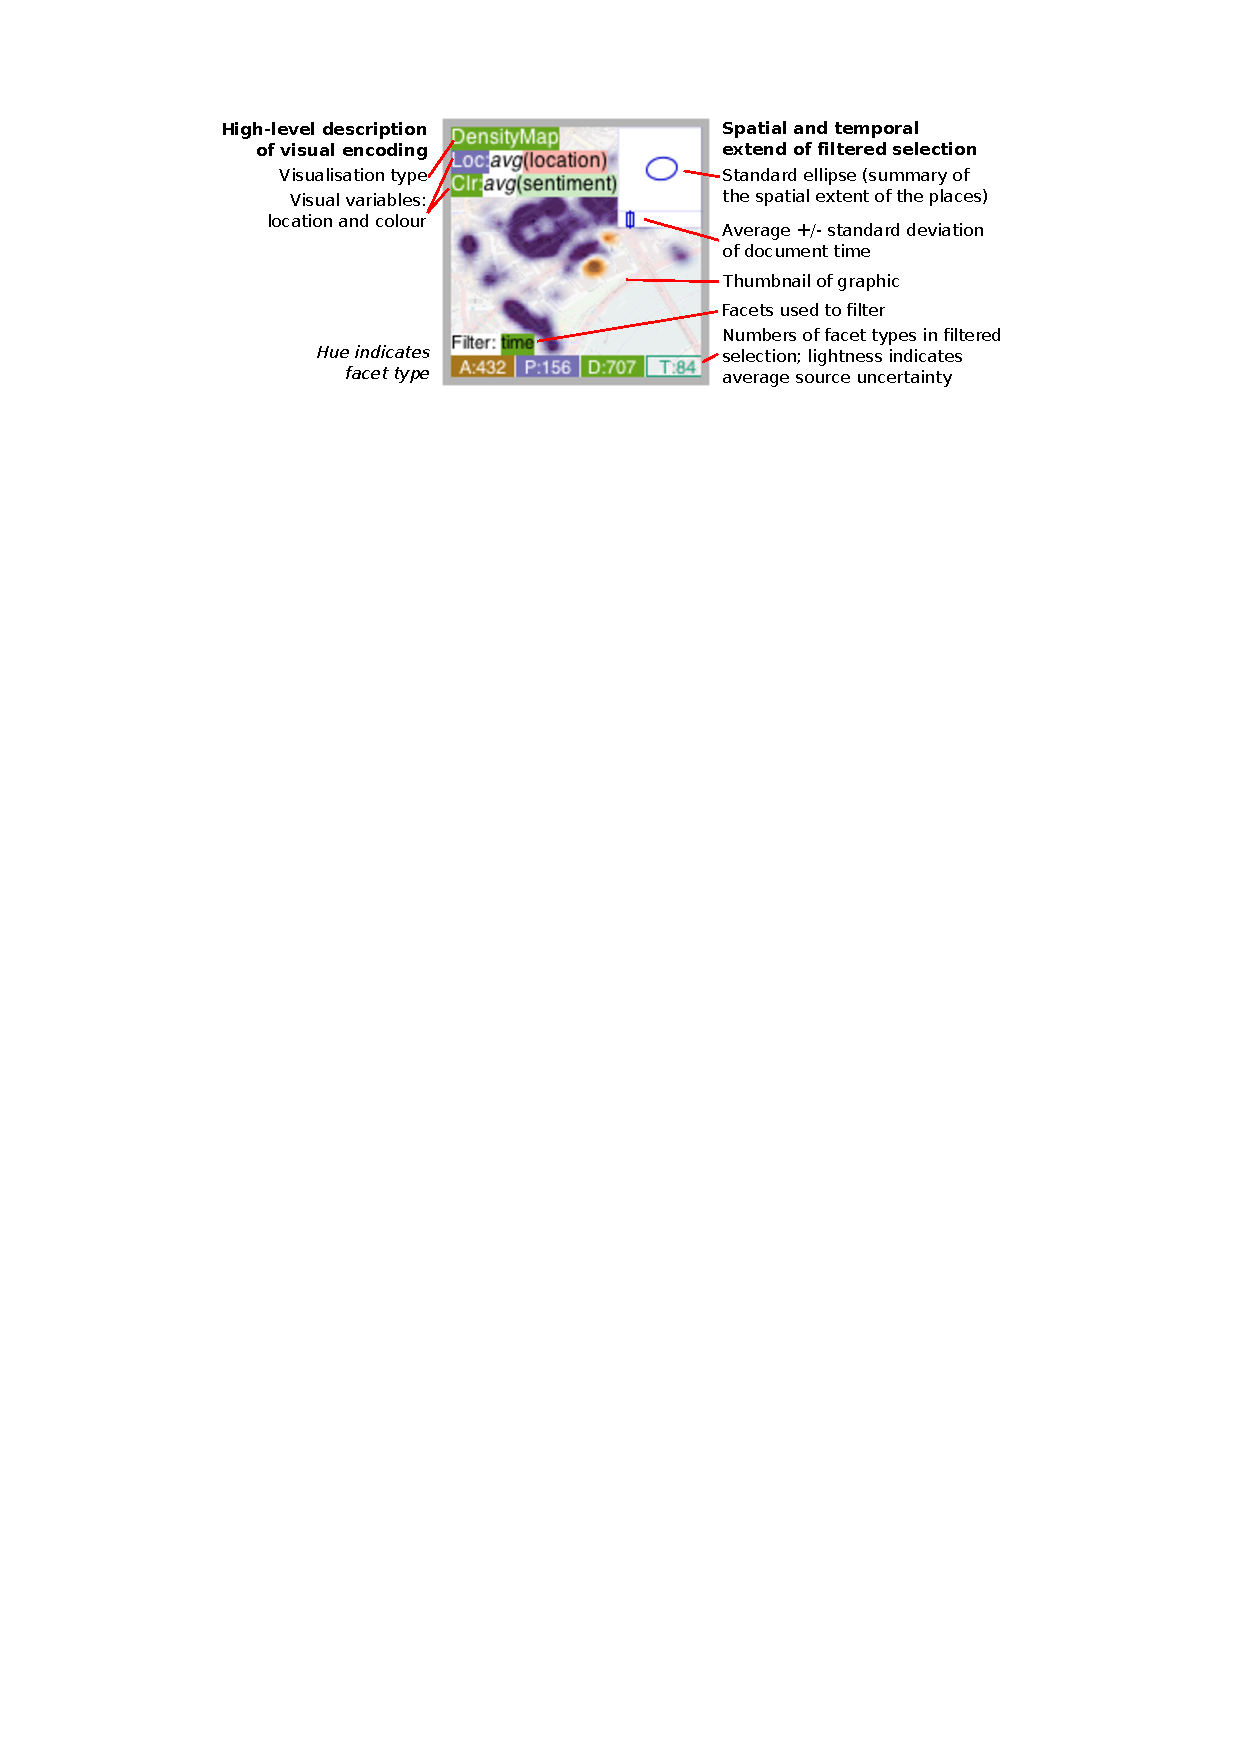
\includegraphics[width=\columnwidth]{thumbnail-encoding}
	\caption[Visualization thumbnails]{Visualization thumbnails with additional information about the filtering used, the characteristics of the filtered subset of data and the visual encoding. \is{Walker2013}}
	\label{fig:lr-thumbnail-encoding}
\end{figure}

It may be necessary to apply pre- and post-processing adjustments to make the visualization thumbnails more recognizable~\cite{Heer2008}. For example, high-frequency visual elements that are not helpful in a small size such as gridlines and element borders can be removed to prevent their domination in the resulting thumbnail. As a result of down-sampling techniques, colors of data items may be different from them in the original visualization. Therefore, readjusting the color to match its intended value could help users recognize the visualizations they saw in the past.

The default snapshot may also be an imperfect representation of a web page, especially if it contains a lot of text. Teevan~et~al.~\cite{Teevan2009} propose an automatic method to produce a thumbnail improving its recognition. The thumbnail consists of three components: salient text at the top-left hand corner, a salient image below the text, and a watermarked logo superimposed at the bottom left hand corner of the image. The salient text contains about 20 first characters of the web page title. The salient image and the branding logo are chosen from the page using machine learning. \autoref{fig:lr-enhanced-thumbnail} shows such a thumbnail.

\begin{figure}
	\centering
	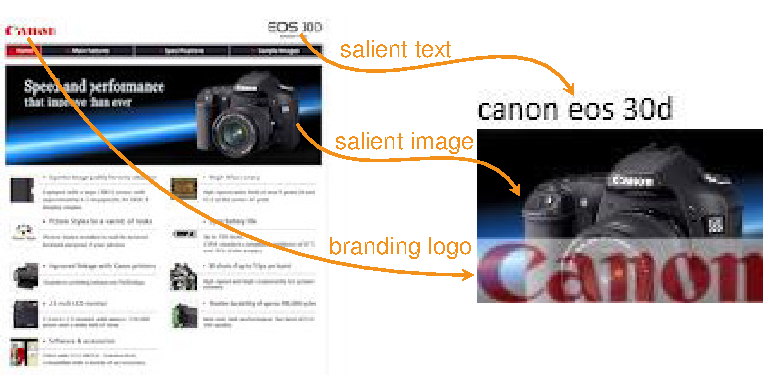
\includegraphics[width=.8\columnwidth]{enhanced-thumbnail}
	\caption[An enhanced web thumbnail]{An enhanced web thumbnail (right) as a composite of salient text, a salient image and a branding logo. \is{Teevan2009}}
	\label{fig:lr-enhanced-thumbnail}
\end{figure}

Besides recognizing previous states, seeing the difference between a state and the one before it is also important in understanding the analysis process. One approach is to highlight the difference between two consecutive states. The changes may only happen at a small portion of the entire interface. Therefore, showing only that area in both states could help users quickly identify the difference.

\subparagraph{Layout} Linear and branching layouts are commonly used to position actions and states, depending on the structure of data capture.

\textbf{Linear Layout} --- Provenance data usually contains an inherent \emph{time} attribute, recording when an action happened. An approach that emphasizes on the order of actions is to show them as a linear sequence of items like a comic strip~\cite{Kurlander1988,Meng1998}. This layout facilitates visual scanning of past actions, allowing users to quickly understand the analysis process. \autoref{fig:lr-comic-strip} shows such a layout.

\begin{figure}
	\centering
	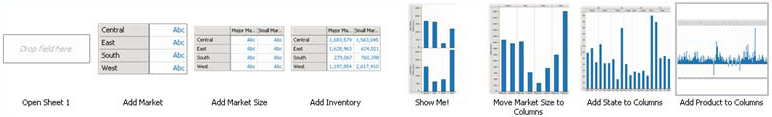
\includegraphics[width=\columnwidth]{comic-strip}
	\caption[Comic strip layout]{Comic strip layout. A sequence of past actions in chronological order. \is{Heer2008}}
	\label{fig:lr-comic-strip}
\end{figure}

\begin{figure}
	\centering
	\subcaptionbox{Time-point provenance data. User annotations are positioned along a time axis at when their associated events happen. \is{Gotz2006}\label{fig:lr-continuous-timeline-1}}[\columnwidth]{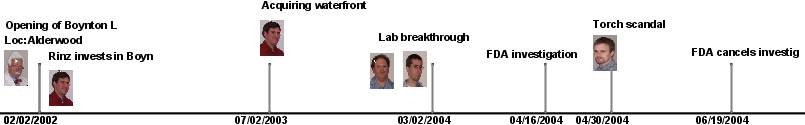
\includegraphics[width=\columnwidth]{continuous-timeline-1}}
	
	\vspace{.5\baselineskip}
	
	\subcaptionbox{Interval provenance data. User actions are shown as horizontal bars a long a time axis covering their durations. \is{Plaisant1999}\label{fig:lr-continuous-timeline-2}}[\columnwidth]{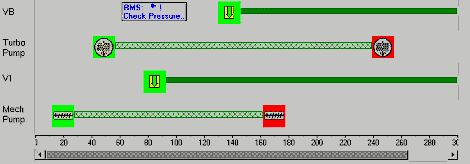
\includegraphics[width=\columnwidth]{continuous-timeline-2}}
	\caption{Timeline layout for visualizing the analysis process.}
\end{figure}

If the absolute timestamps of actions are of interest, a continuous timeline~\cite{Derthick2001} is a more suitable layout. Actions are positioned along the time axis at when they happen (\autoref{fig:lr-continuous-timeline-1}) or during which they last (\autoref{fig:lr-continuous-timeline-2}). The time axis can be either horizontal or vertical~\cite{SandboxTimeline2012}. The layout algorithms found in these provenance timelines are quite naive. POLESTAR~\cite{Pioch2006} and the timeline from Jigsaw~\cite{Liu2010} require manual rearrangement of the events from users to solve the overlapping problem. The timeline from nSpace2 Sandbox~\cite{SandboxTimeline2012} shows events at the exact time when they happen without considering possible intersection between of them.

Another approach is to use both the horizontal and vertical axes to represent time. BrowseLine~\cite{Hoeber2009} uses the vertical axis for \emph{macro-time} and the horizontal axis for \emph{micro-time}, similar to stem-and-leaf plots. More specifically, a two-dimensional timeline (\autoref{fig:lr-timeline-2d}) is divided into rows, each for a macro time-slot, such as one hour. In each row, events happening within that hour are positioned along the horizontal axis without considering their absolute timestamps. This design assumes that users may only remember roughly when events happen, thus absolute positioning in the vertical axis facilitate them in recognizing past events. Moreover, relative positioning in the horizontal axis could help pack more events and prevent overlapping.

\begin{figure}
	\centering
	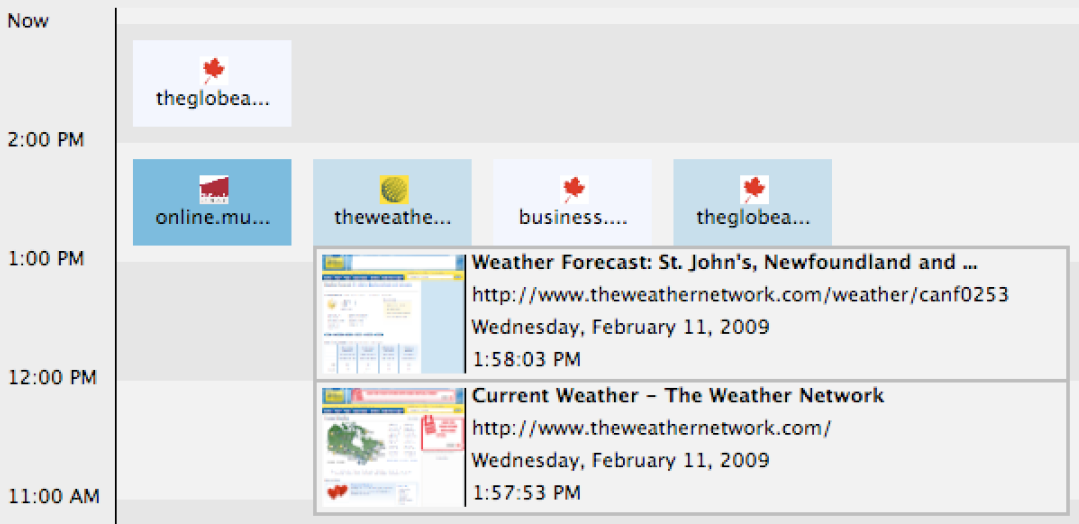
\includegraphics[width=\columnwidth]{timeline-2d}
	\caption[Two-dimensional timeline]{2D timeline. The vertical axis represents macro-time, whereas the horizontal axis represents micro-time. Events within a macro time-slot are positioned in chronological order as a comic strip. \is{Hoeber2009}}
	\label{fig:lr-timeline-2d}
\end{figure}

\textbf{Branching Layout} --- Many sensemaking systems allow users to revisit their past states such as through undo/redo features or backward/forward in web browsers. From a past state, if the user performs a new action, it should be recorded in a new branch forking from that state. This branching history is typically visualized with a tree layout to represent the logic of the analysis process effectively. In such a tree, nodes represent a summary of system states, and edges represent actions that transition the system from one state to another. Examples can be found in many provenance-enabled systems in different fields including scientific visualization~\cite{Ma1999}, information visualization~\cite{Dunne2012}, visual analytics~\cite{Kadivar2009} and browser history~\cite{Ayers1995}. \autoref{fig:lr-tree-prov} shows such a provenance tree in a scientific visualization.

\begin{figure}
	\centering
	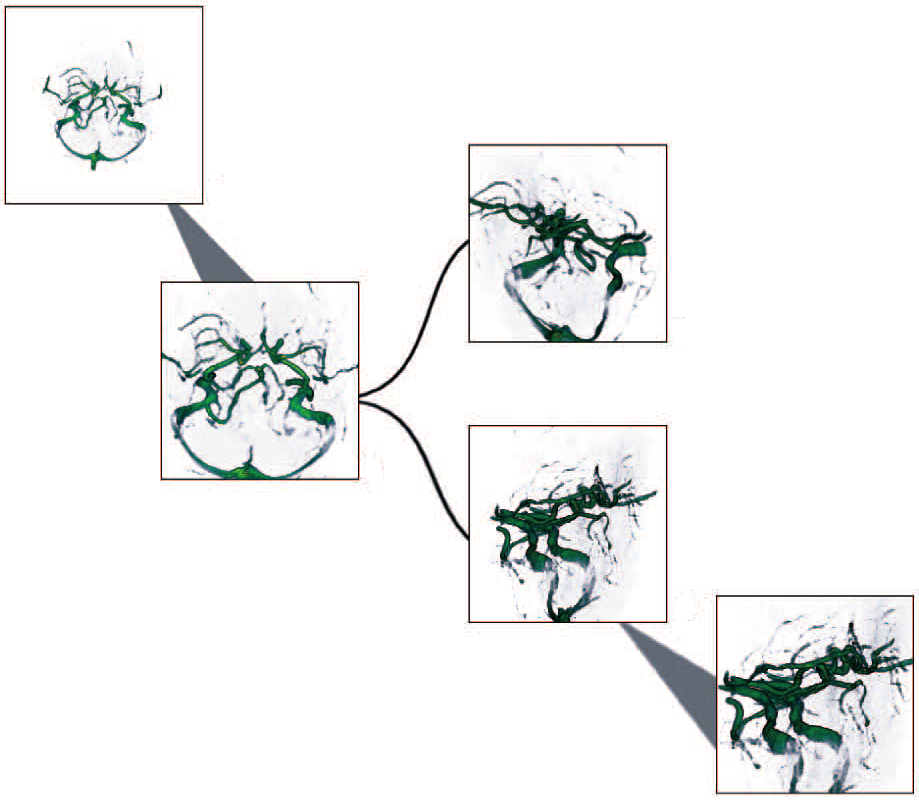
\includegraphics[width=.6\columnwidth]{tree}
	\caption[Tree visualization for branching analysis process]{Tree visualization for branching analysis process. Nodes are thumbnails of past visualization states and links are transforming actions. \is{Jankun-Kelly2007}}
	\label{fig:lr-tree-prov}
\end{figure}

% Time encoding
In a tree layout, the order of actions can be inferred through the direction of edges. Moreover, exact time gap between actions can also be visually encoded into the visualization. VisTrails~\cite{Bavoil2005} color-codes the background of nodes according to their creation time (\autoref{fig:lr-tree-time-1}). Aruvi~\cite{Shrinivasan2008} uses the length of edges to represent the relative time gap between two states (\autoref{fig:lr-tree-time-2}).

\begin{figure}
\centering
\subcaptionbox{Node backgrounds are color based on time. \is{UniversityofUtah2012}\label{fig:lr-tree-time-1}}{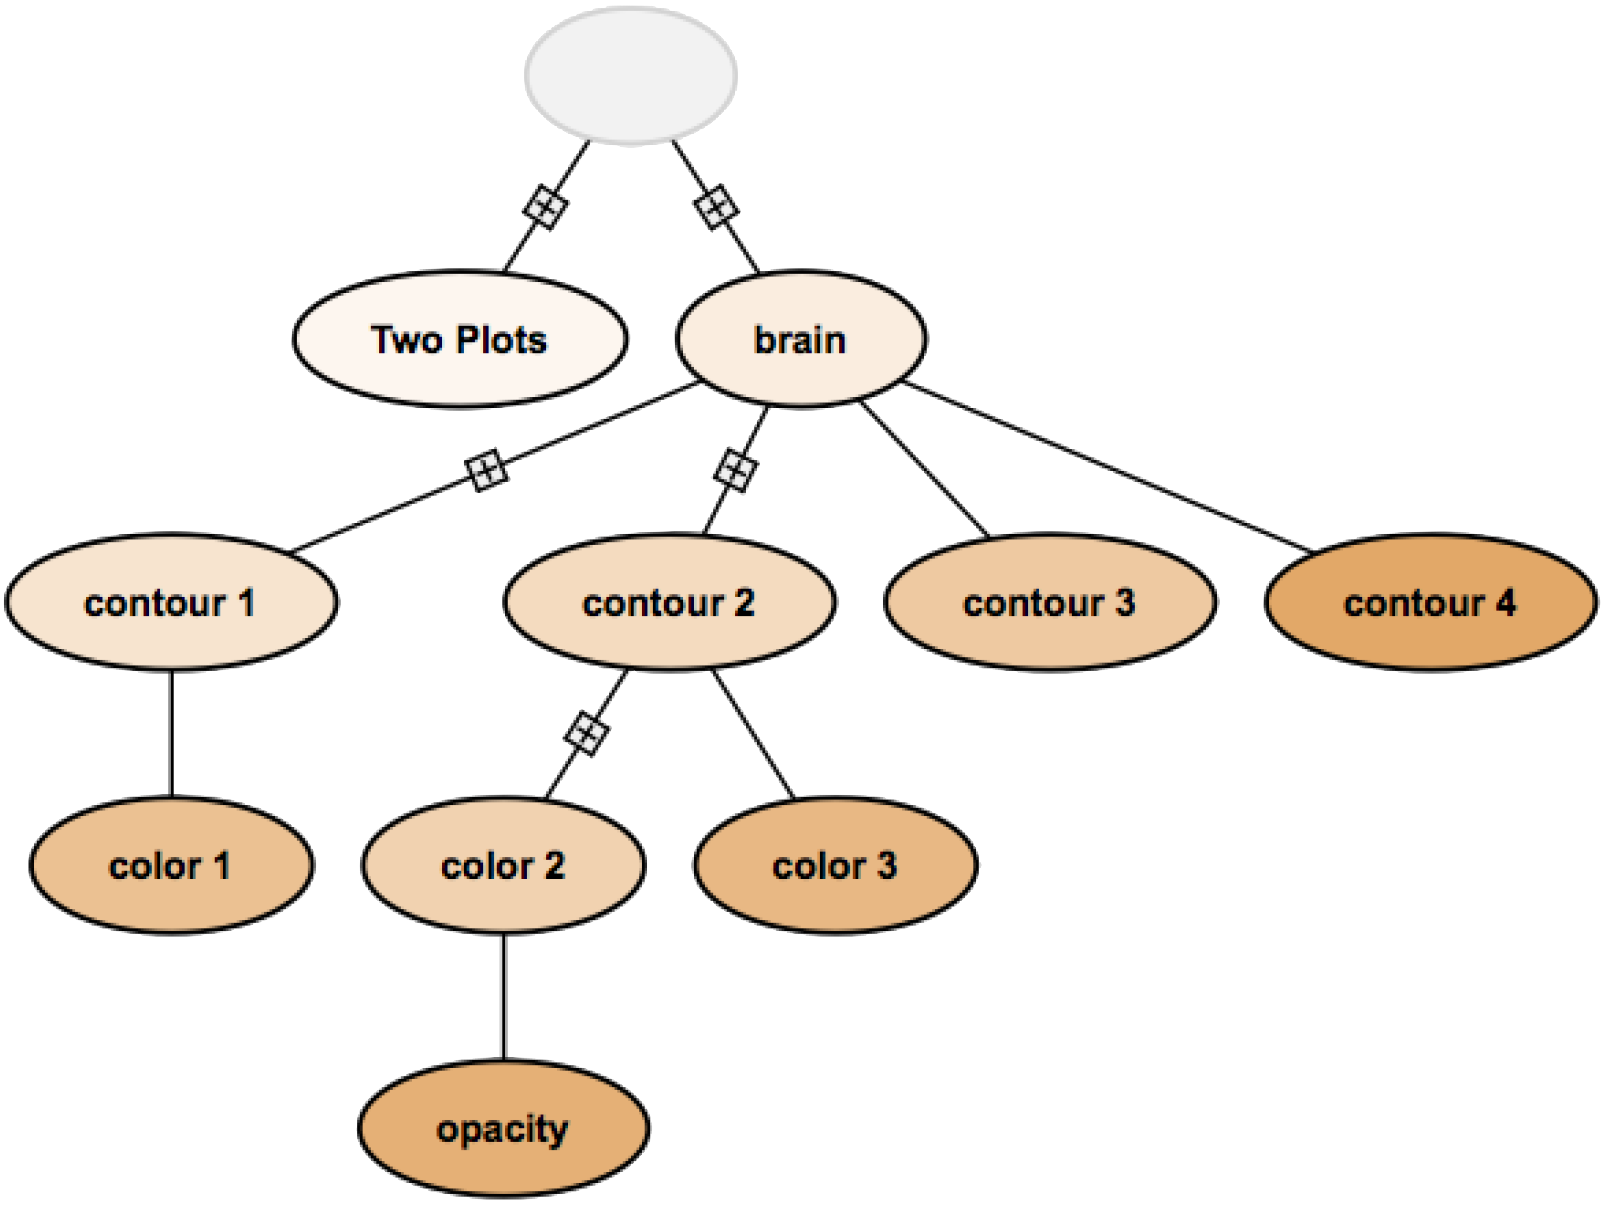
\includegraphics[height=0.21\columnwidth]{tree-time-1}}
\hfill
\subcaptionbox{The edge length between two nodes represents the interval between them. \is{Shrinivasan2008}\label{fig:lr-tree-time-2}}{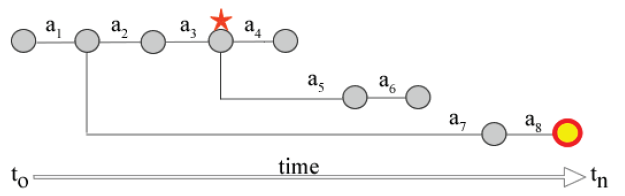
\includegraphics[height=0.21\columnwidth]{tree-time-2}}
\caption{Encoding temporal information into provenance trees.}
\end{figure}

% Other variations
The diagonal arrangement of tree as in~\autoref{fig:lr-tree-time-1} may consume a lot of space. One approach is to use only horizontal and vertical edges as in~\autoref{fig:lr-tree-time-2}. Another approach is to display only the path that led to the currently active  visualization~\cite{Klemmer2002}, and make other paths expanded on demand. \autoref{fig:lr-inline-history} shows such an example.

\begin{figure}
\centering
\subcaptionbox{Branched history. The user first performed actions $A$, $B$, $C$, $D$ and $E$, then undone to $D$, $C$ and $B$, then performed new actions $F$ and $G$.  \label{fig:lr-inline-history-1}}{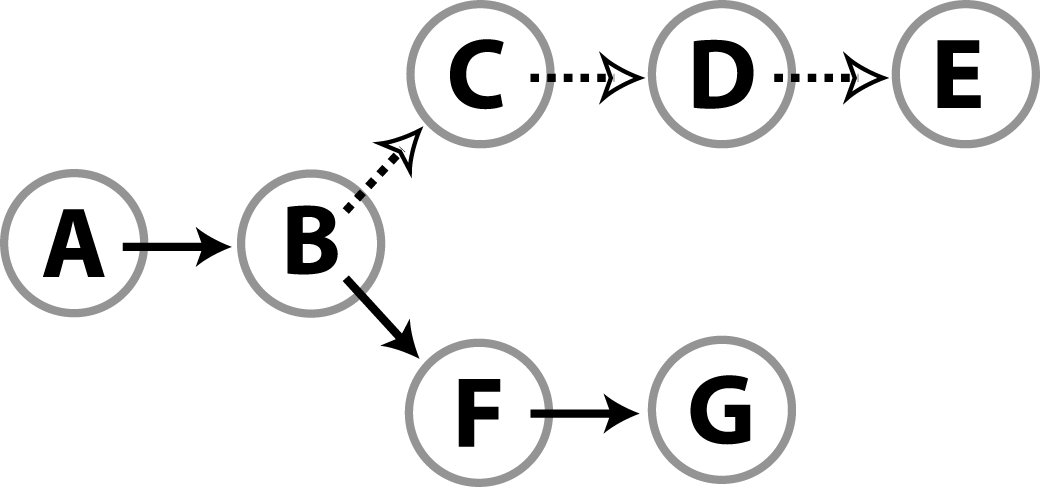
\includegraphics[height=.178\columnwidth]{inline-history-1}}
\hfill
\subcaptionbox{Inline branching history representation. Top: displaying the current path. Bottom: displaying the full history; actions not part of the current path are placed between brackets. \label{fig:lr-inline-history-2}}{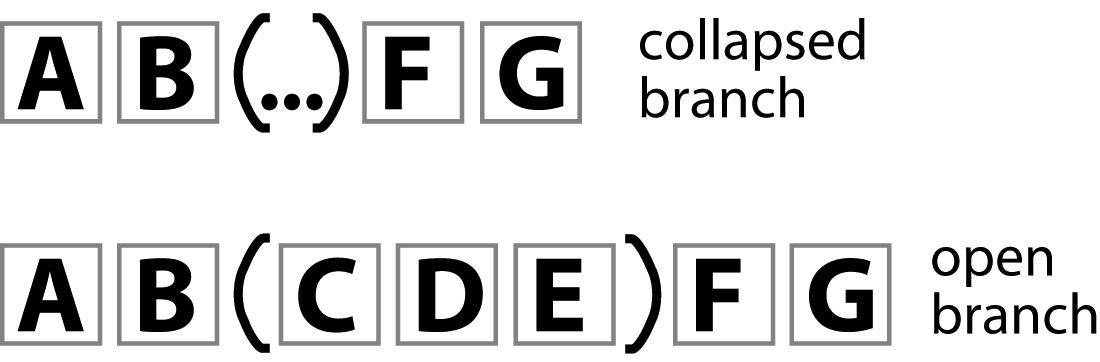
\includegraphics[height=.188\columnwidth]{inline-history-2}}
\caption[Branching layout for tree visualization of the analysis process]{Branching layout for tree visualization of the analysis process. \is{Klemmer2002}}
\label{fig:lr-inline-history}
\end{figure}

% Interaction for scalability
Interaction is also commonly used to address the scalability issue. Zooming and panning enable users to see the overview of the analysis process and navigate to the part of interest~\cite{Dunne2012}. Collapsing and expanding branches of the tree on demand can also help reduce its size and avoid distraction~\cite{Bavoil2005}. Distortion techniques may help users quickly navigate and focus on more relevant states and actions~\cite{Meng1998}. Another technique for compressing the provenance tree and improving user understanding is \emph{action chunking}~\cite{Heer2008}: a sequence of related actions may be better represented as a single higher-level activity. For example, a quick succession of sort or filter actions likely indicate a multi-step configuration of the view and can be chunked together.

Typically, provenance data is shown in a separate view, linked with other data views of the visualization system~\cite{Shrinivasan2008,Heer2008,Pike2009,Kadivar2009}. However the system can also be used as a single item of the provenance view. For instance, in GraphTrail~\cite{Dunne2012}, a single-view visualization system, when the visualization is changed (e.g., changing attribute mapping in a bar chart), it creates a new view containing that visualization and links with the current view. This is similar to how normally the provenance view is developed; however, GraphTrail makes the entire exploration space become the provenance view. Moreover, each history item is not a thumbnail, but a fully interactive visualization. Through zooming and panning, users can switch between a close examination of individual system states (\autoref{fig:lr-detail}) and an overview of the analysis structure (\autoref{fig:lr-overview}). An extra overview window as in overview-and-detail technique~\cite{Cockburn2008} could be useful in search and navigation in a large space.

\begin{figure}
\centering
\subcaptionbox{Zooming in to work on the active visualization.\label{fig:lr-detail}}[0.33\columnwidth]{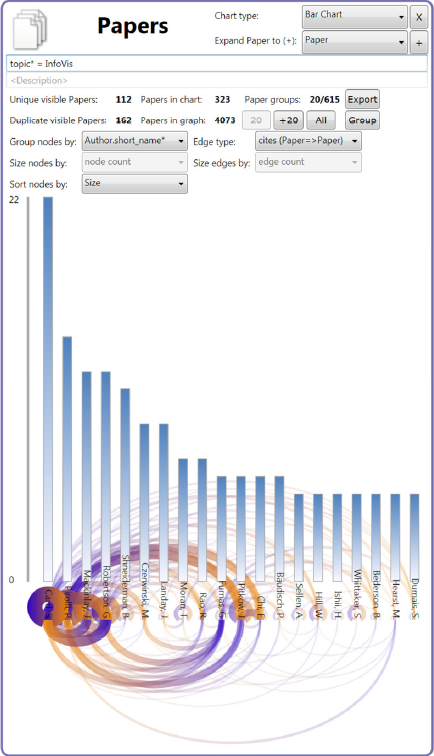
\includegraphics[height=0.5\columnwidth]{GraphTrail-detail}}
\hfill
\subcaptionbox{Zooming out to see an overview as the history of the exploration process.\label{fig:lr-overview}}[0.57\columnwidth]{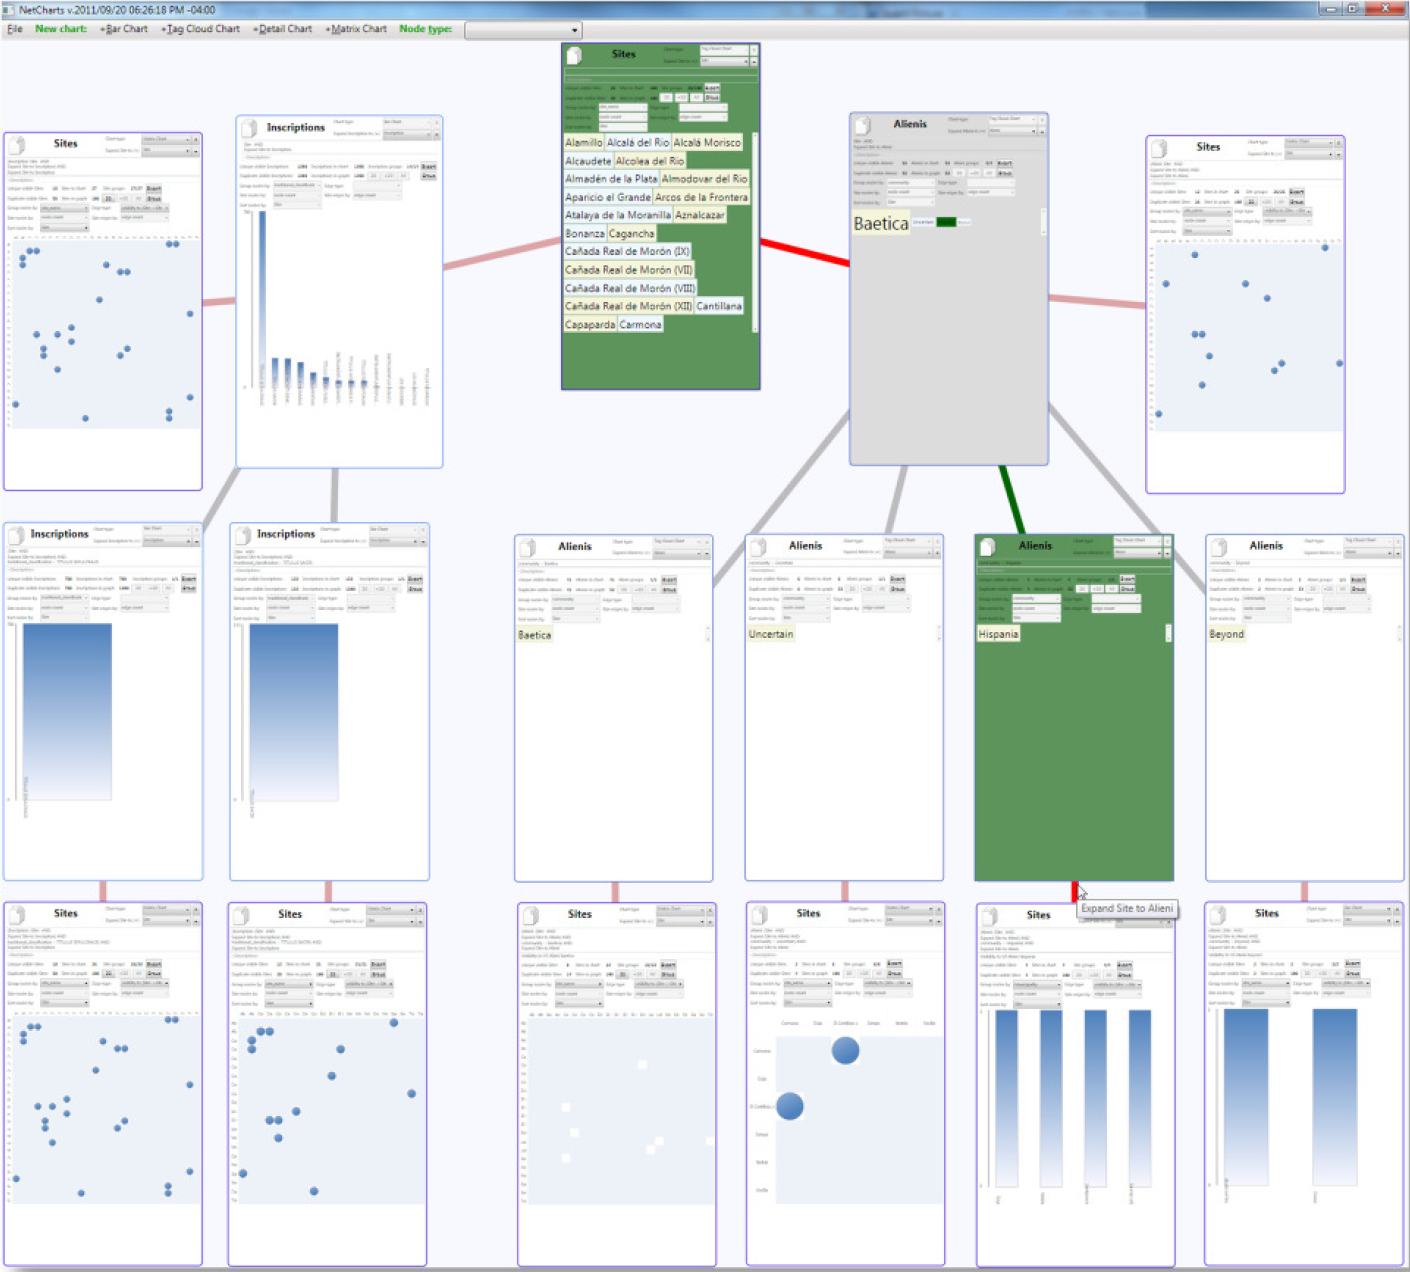
\includegraphics[height=0.5\columnwidth]{GraphTrail-overview}}
\caption[Unification of the exploration view and the history view]{Unification of the exploration view and the history view. \is{Dunne2012}}
\end{figure}

\subsubsection{Sub-Tasks and Tasks}
Tasks and sub-tasks provide important clues to the purpose and rationale underlying the sensemaking process. However, they are largely part of users' thinking, which a visual analytics system does not have direct access to. Also, the time window to capture such information is very limited. Even the users themselves may forget what they were doing after a while, making it difficult to recover the analytic provenance information. Therefore, capturing high-level tasks and sub-tasks is one of the biggest challenges in analytic provenance capture.

Existing approaches to capture high-level analytic provenance can be broadly categorized into manual and automatic methods. The \emph{manual} methods rely on users recording their analysis processes and sensemaking tasks, whereas the \emph{automatic} methods try to infer the higher level tasks and sub-tasks from lower level events and actions. Even though the manual approaches are usually more accurate, they can distract users from the actual analysis tasks, which may discourage users from recording analytic provenance. Alternatively, the automatic approaches do not introduce interruption to the sensemaking process, but their capability of inferring semantic-rich analytic provenance information is limited~\cite{Gotz2009}. Individual differences also introduce additional challenges to designing a robust algorithm for the inferring process. Users' knowledge and experience have a considerable impact on the way they conduct analyses. As a result, the sensemaking process can vary significantly from users to users, even with the same dataset and analysis task.

\subparagraph{Manual}
%User annotation is one of the most common forms in manual capture. Users create \emph{notes} or \emph{annotations} that are associated with certain data, analysis result, and/or visualization~\cite{Heer2009,Walker2013}. The content of such a ``note'' is not limited to findings or discoveries; it can also include the thinking that leads to a finding or the relationship between findings. \emph{Data-aware annotation}~\cite{Heer2008a} links a finding and the associated visualization to the underlying data used to produce it, which makes it possible to conduct further analysis if necessary.

Tasks and sub-tasks can be captured by allowing the user to externalize them manually. A common form of reasoning externalization is to allow users to write down their thinking. It could be a free note~\cite{Shrinivasan2008} or a description of a user bookmarked visualization~\cite{Heer2009,Walker2013}. Alternatively, users can annotate directly on the visual bookmark using standard graphical editing features such as circling on interesting patterns (\autoref{fig:lr-annotation-1} -- Top) or hand drawing on a suspicious trend (\autoref{fig:lr-annotation-1} -- Bottom). To make the annotation more meaningful across multiple views, the selection should be aware of the data involved in it~\cite{Heer2008a}. For example, in \autoref{fig:lr-annotation-2}, the annotation in the top view also makes the data items in the bottom view get annotated using the same selection query. Data-aware annotations allow users to see the data of interest remained across different views.

\begin{figure}
\centering
\subcaptionbox{Geometric annotation.\label{fig:lr-annotation-1}}{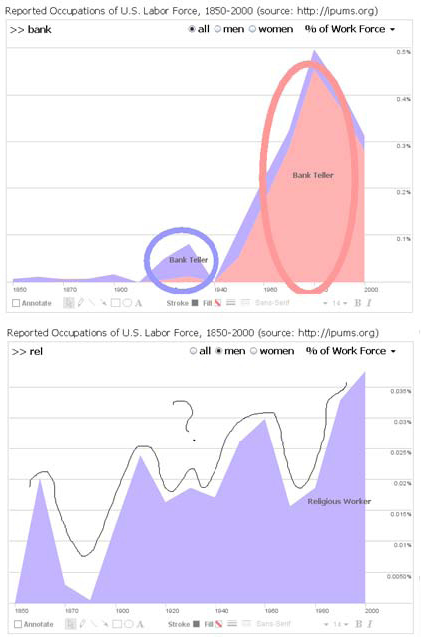
\includegraphics[height=0.6\columnwidth]{annotation-1}}
\hspace{1cm}
\subcaptionbox{Data-aware annotation.\label{fig:lr-annotation-2}}{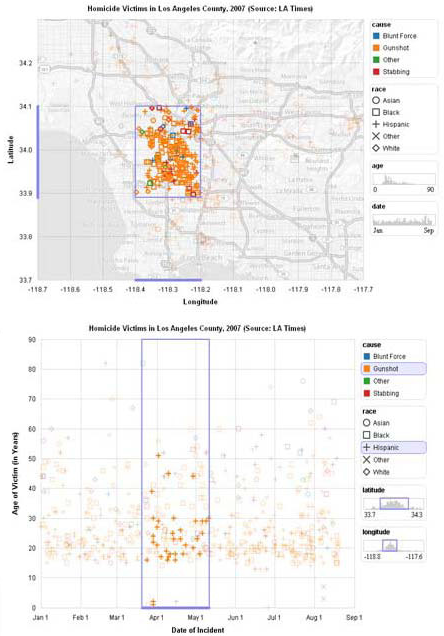
\includegraphics[height=0.6\columnwidth]{annotation-2}}
\caption[User annotation of bookmarked visualization]{User annotation of bookmarked visualization as a form of manual capture of tasks and sub-tasks. \is{Heer2012}}
\label{fig:lr-annotation}
\end{figure}

Even though an individual note only represents a fraction of the analytic provenance, it is possible to provide a reasonably good overview of the sensemaking process if a number of notes and the connections between them are captured. For example, the \emph{Scalable Reasoning System} ~\cite{Pike2009} allows users to record their discoveries of interesting patterns about the data, then specify their causal relationships by drawing links, and generate hypotheses based on these artifacts. For example, users can show connections between a hypothesis and its evidence by drawing links, and spatially separate the evidence into a supporting group and a counter group, facilitating further comparison. These interactive features are known to help users produce more critical thinking in their analyses~\cite{Sedig2013}.  \autoref{fig:lr-reasoning-simple-note} shows such a diagram produced with user notes and \autoref{fig:lr-reasoning-diagram-SRS} shows such a more formal diagram with different reasoning roles.

\begin{figure}
\centering
\subcaptionbox{A diagram of user notes showing their thoughts. \is{Shrinivasan2008}\label{fig:lr-reasoning-simple-note}}{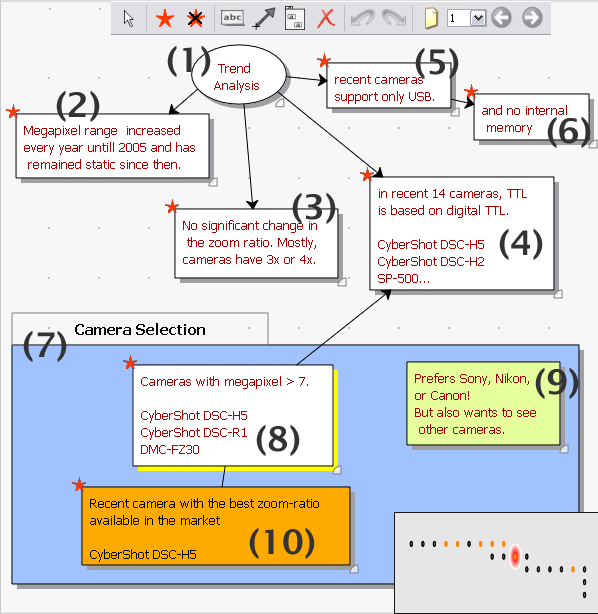
\includegraphics[height=0.42\columnwidth]{reasoning-simple-note}}
\hfill
\subcaptionbox{A formal reasoning diagram with nodes having different roles: evidence, casual relationship, assumption and hypothesis. \is{Pike2009a}\label{fig:lr-reasoning-diagram-SRS}}{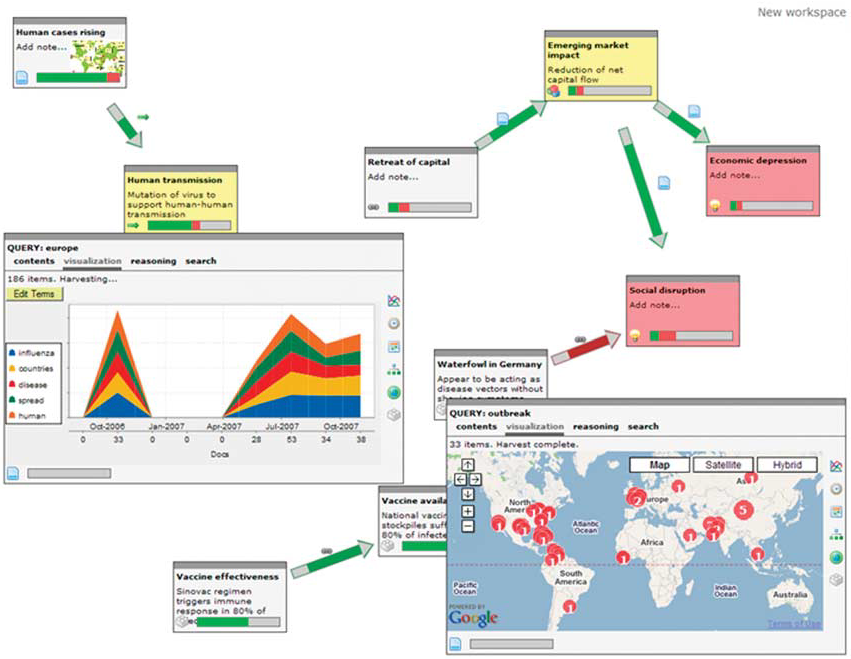
\includegraphics[height=.42\columnwidth]{reasoning-diagram-SRS}}
\caption{Task and subtask visualization.}
\end{figure}

% Formal reasoning
More analytical reasoning methods have also been integrated to visual analytics systems to allow users to perform complex analyses with their externalized thoughts. POLESTAR~\cite{Pioch2006} supports argument structuring, based on methods for analyzing legal documents such as the Toulmin model of argument~\cite{Toulmin2003}. To help validate a hypothesis, it organizes arguments as a tree structure of claims, each supported by at least one piece of evidence. A claim can have its supporting sub-claims and can also have rebuttals that weaken or restrict their force. \autoref{fig:lr-reasoning-argument-editor} shows such an argument tree. Sandbox~\cite{Wright2006} supports analysis of competing hypotheses -- a judgment method that requires careful weighing of alternative explanations~\cite{Heuer1999}. It allows users to add multiple hypotheses, each with supporting or contradictory evidence. These pieces of evidence are weighted by the users and summarized in a visual matrix, enabling the users to effectively make a decision without having to remember and analyze in their minds. \autoref{fig:lr-reasoning-ACH} shows an example of this support.

\begin{figure}
\centering
\subcaptionbox{Argument tree with claims, sub-claims, and facts. \is{Pioch2006}\label{fig:lr-reasoning-argument-editor}}{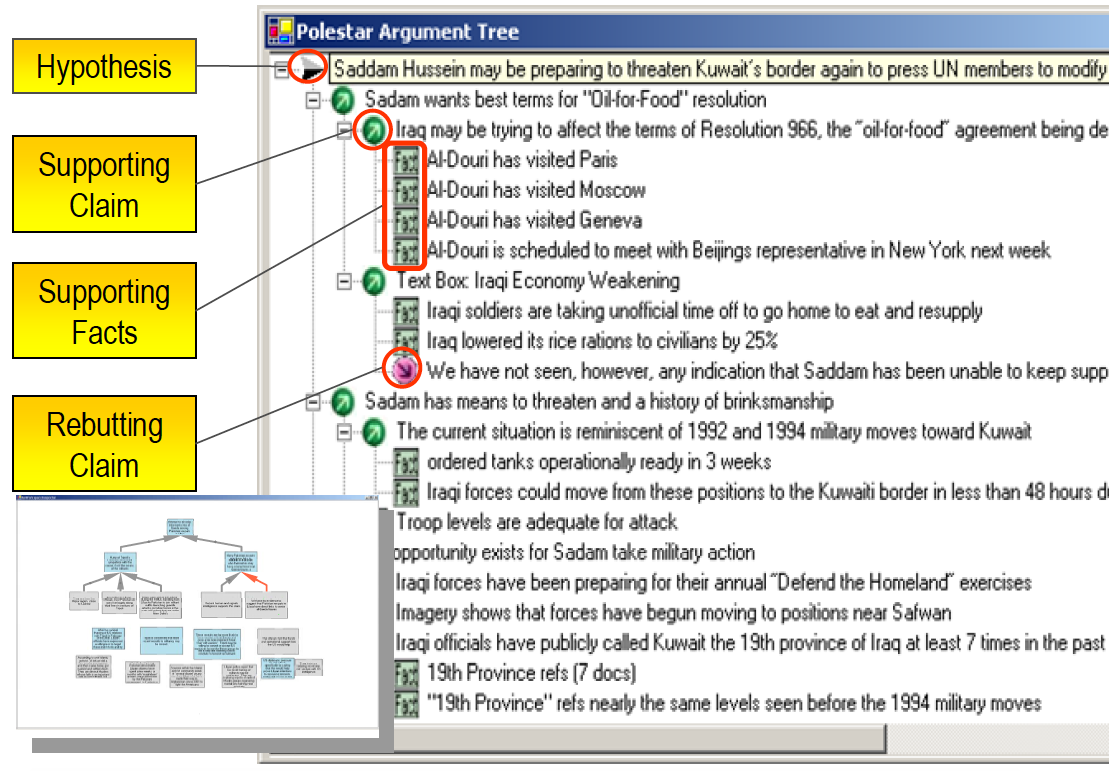
\includegraphics[height=0.3\columnwidth]{reasoning-argument-editor}}
\hfill
\subcaptionbox{Analysis of competing hypotheses with weighted supporting/counter evidence. \emph{Image source: a video snapshot of~\cite{Wright2006}.}\label{fig:lr-reasoning-ACH}}{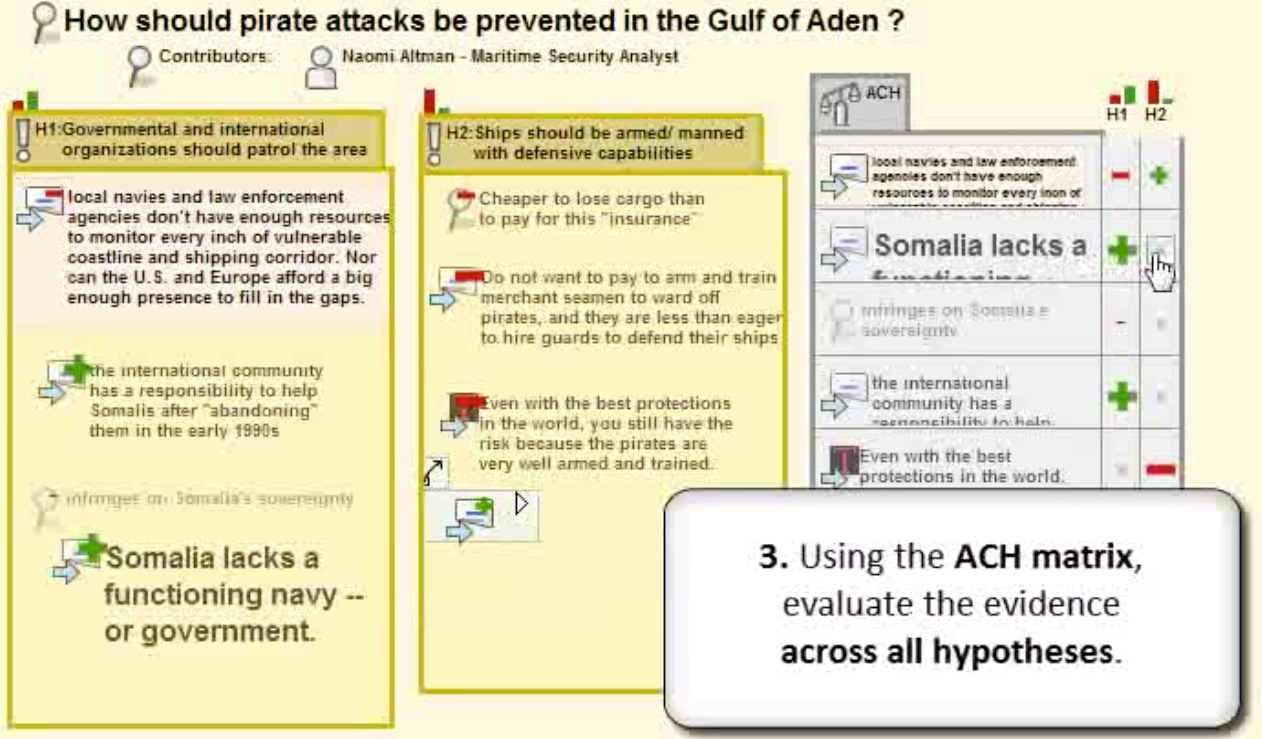
\includegraphics[height=0.3\columnwidth]{reasoning-ACH}}
\caption[Analytical support for the sensemaking process]{Analytical support for the sensemaking process with externalized thinking artifacts.}
\label{fig:lr-reasoning}
\end{figure}

Despite all the aforementioned benefits, manual capture is only useful when users are willing to take notes, which sometimes can be perceived as distractions. Two common strategies to alleviate this include minimizing interruption/cognitive effort~\cite{Hong2008} and providing immediate benefits to the sensemaking task such as planing exploratory analysis for complex tasks~\cite{Lunzer2014}. However, currently there is a lack of general design guidelines for how to achieve them, and there are few user studies evaluating how effective they are, in terms of both the benefits they bring and the potential cognitive cost they can introduce.

\subparagraph{Automatic}
One of the main disadvantages of manual capture is the requirement of direct input from users. Automatic approaches try to address this by inferring higher level analytic provenance from what can be automatically captured, which are events and actions. This turns out to be a difficult challenge. An experiment studied how much of a user's reasoning process can be recovered from user action information~\cite{Dou2009}. A domain-specific sensemaking task was used for participants to solve, and experts were recruited to analyze the their action logs. Higher-level analytic provenance manually inferred from the logs was compared with the ground truth obtained through interview. The results showed that 79 percent of the findings, 60 percent of the methods, and 60 percent of the strategies were recovered correctly. The accuracy is not high even in such a constrained setting with domain experts doing the inference. Given the diversity of data and analysis involved in the sensemaking and the difficulty of replicating expert knowledge in a computer system, the probability of having a generic technique that can accurately infer semantic-rich analytic provenance information for a variety of analysis tasks can be low.

%Instead, existing methods either constrain the problem/analysis domain or aim for less semantically rich analytic provenance. By limiting the choice of data and analysis/visualization, an inference algorithm has better chance to make the right guess. However, even within a specific domain, the types of data and analyses involved are still of very large amount. Also, being limiting on the data and analysis can constrain the system capability, having a negative impact on the sensemaking task.

Given the difficulty of inferring task/sub-task information, a few methods target less semantic-rich provenance. One example is \emph{action chunking}, which identifies a group of actions that are likely to be part of the same sub-task, without knowing what the sub-task is. Such approaches apply heuristics to infer patterns from action logs based on repeated occurrence and proximity in data/visualization space or analysis time. For instance, one simple heuristic is about the action structure of a sub-task: a series of ``exploratory'' actions (e.g., sort, filter, zoom, etc) followed by an ``insight'' action (e.g., bookmark and annotation)~\cite{Gotz2009}. However, it may only work if the user spends time on doing bookmark and annotation, which may be impractical as discussed previously. Another example is to extract sub-tasks from a sequence of actions based on predefined patterns~\cite{Gotz2009b}. One such pattern is ``scan'' defined as a series of ``inspect'' actions on similar data objects. For instance, in travel planning, when the user opens several hotels to check their price, he or she might want to scan or compare price of those hotels. This method is later extended to monitor user behavior for implicit signals of user intent and uses the information to suggests alternative visual designs.

\subsection{Summary}
This section reviews research on analytic provenance, characterized by the four-level model by Gotz and Zhou~\cite{Gotz2009}. It covers the capture and visualization of all levels: event, action, sub-task and task. It is more straightforward to capture events and actions; however, they contain few semantics compared to sub-tasks and tasks. The later two levels are often manually captured through annotation. This thesis applies both manual capture (\autoref{chap:schemaline}) and automatic capture  (\autoref{chap:sensepath}) of the action level, and supports users to gain understanding of the higher levels through visualization of the captured provenance data. Existing visualizations of provenance data are not specifically designed to support the iterative and dynamic nature of sensemaking. They mainly support users to recall and replicate their analyses, recover their performed actions, and present their final analysis results. This thesis focuses on supporting the ongoing and iterative sensemaking by contributing novel visualization techniques to explore complex temporal (\autoref{chap:schemaline} and \autoref{chap:timesets}) and reasoning (\autoref{chap:sensepath} and \autoref{chap:sensemap}) relationships hidden in the sensemaking problem. Literature of temporal and network visualization (to help explore reasoning relationship) will be discussed in the next two sections, respectively.